% Déclaration du type de document (report, book, paper, etc...)
\documentclass[a4paper]{report} 
 
% Package pour avoir Latex en français
\usepackage[utf8]{inputenc}
\usepackage[francais]{babel}
 
% Quelques packages utiles
\usepackage{listings} % Pour afficher des listings de programmes
\usepackage{graphicx} % Pour afficher des figures
\usepackage{amsthm}   % Pour créer des théorèmes et des définitions
\usepackage{amsmath}

% Auteur
\author{Antoine Albertelli -- CVRA}

 
% Titre du document
\title{Utilisation de l'environnement Nios II SBT}

% Début du document
\begin{document}

\maketitle
\tableofcontents
 
\chapter{Installation}
\section{Outils nécessaires}

Les outils nécessaires pour le développement sont :
\begin{itemize}
\item Quartus II Web edition (testé avec la version 11sp1).
\item Nios II Embedded Design Suite (testé avec la version 11sp1).
\item Un client Mercurial (hg sous Linux, TortoiseHG sour Windows).
\end{itemize}

\section{Récupération du code source}
La première étape est de récupérer le code source depuis Bitbucket.
Pour ceci :
\begin{lstlisting}[frame=trBL]
> hg clone http://bitbucket.org/antoinealb
/code-source-carte-robot-2011
\end{lstlisting}

Un dossier nommée code-source-carte-robot-2011 a maintenant été créé et contient le code du robot.

\textbf{Attention}: Ce dossier doit contenir uniquement les fichiers sources, pas le BSP\footnote{Board Support Package, generé par le Nios II EDS} ni les fichier exécutables !


Plus tard lorsqu'on voudra mettre à jour le code il suffira de faire :
\begin{lstlisting}[frame=trBL]
> hg pull
> hg update
\end{lstlisting}

\section{Création du projet dans le Nios II EDS}

\begin{figure}[h!]
  \centering
    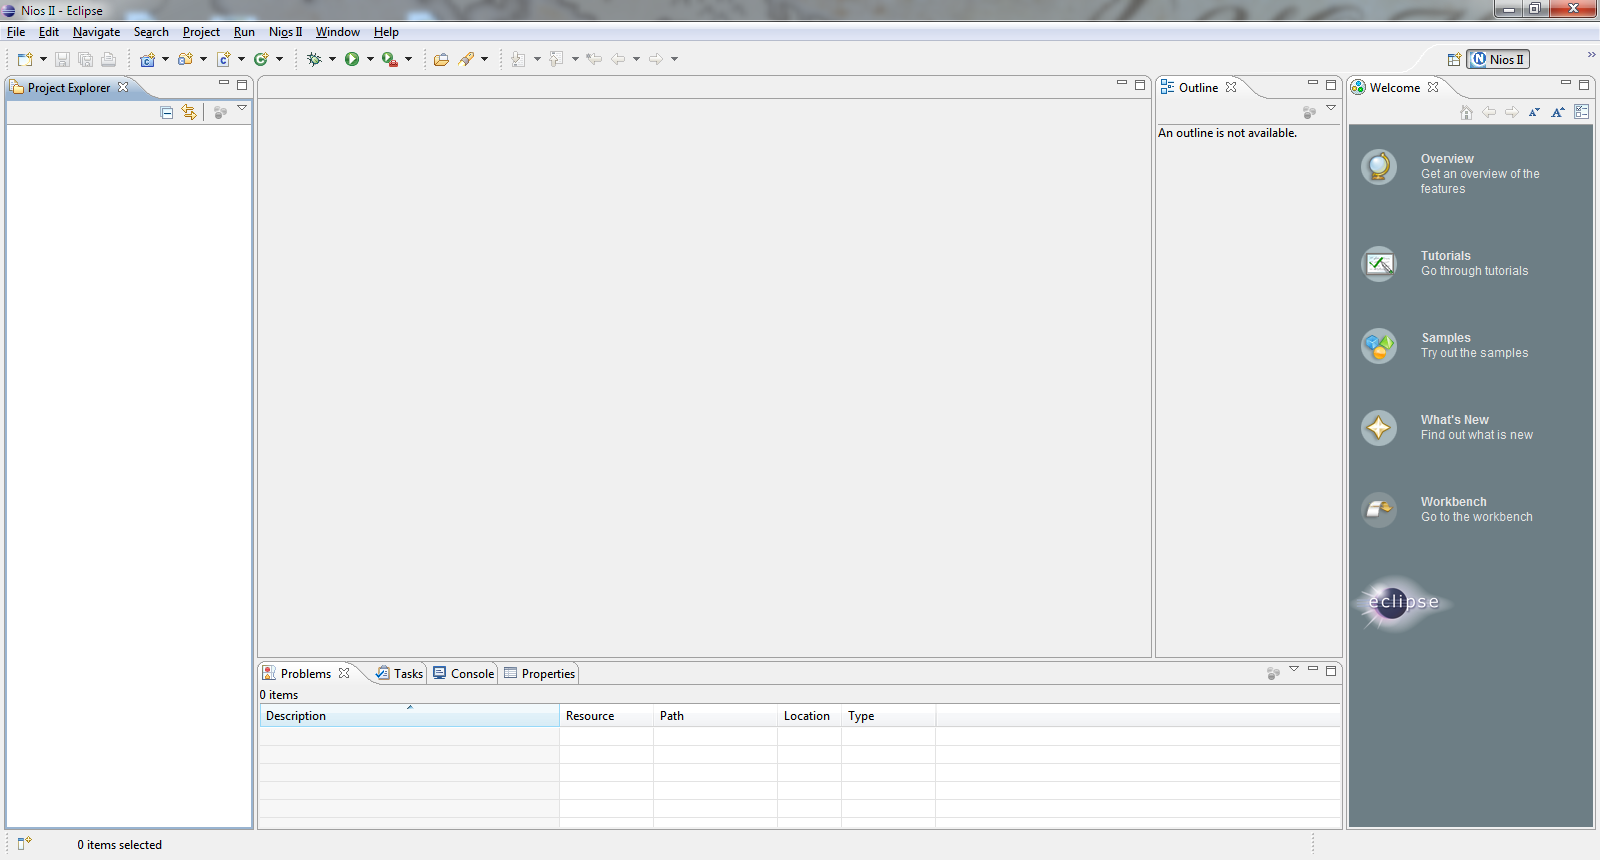
\includegraphics[width=0.8\textwidth]{1}
  \caption{L'environnement de développement Nios II EDS}
\end{figure}

Dans l'environnement de développement, faire "New Application and BSP from template...".
\begin{figure}[h!]
  \centering
    \includegraphics[width=0.8\textwidth]{tuto2}
  \caption{Création du projet. Choisir "Empty project"}
  \label{projectcreation}
\end{figure}
Dans cette fenêtre (fig. \ref{projectcreation}) choisir "Empty Application" comme template et faire "Finish".
Ensuite, aller dans chaque dossier contenant du code source (sauf "tools"), séléctionner les fichier, 
click droit -> "Add to Nios II build". Il faut aussi le faire pour les sous dossiers de "modules".

\begin{figure}[h!]
  \centering
    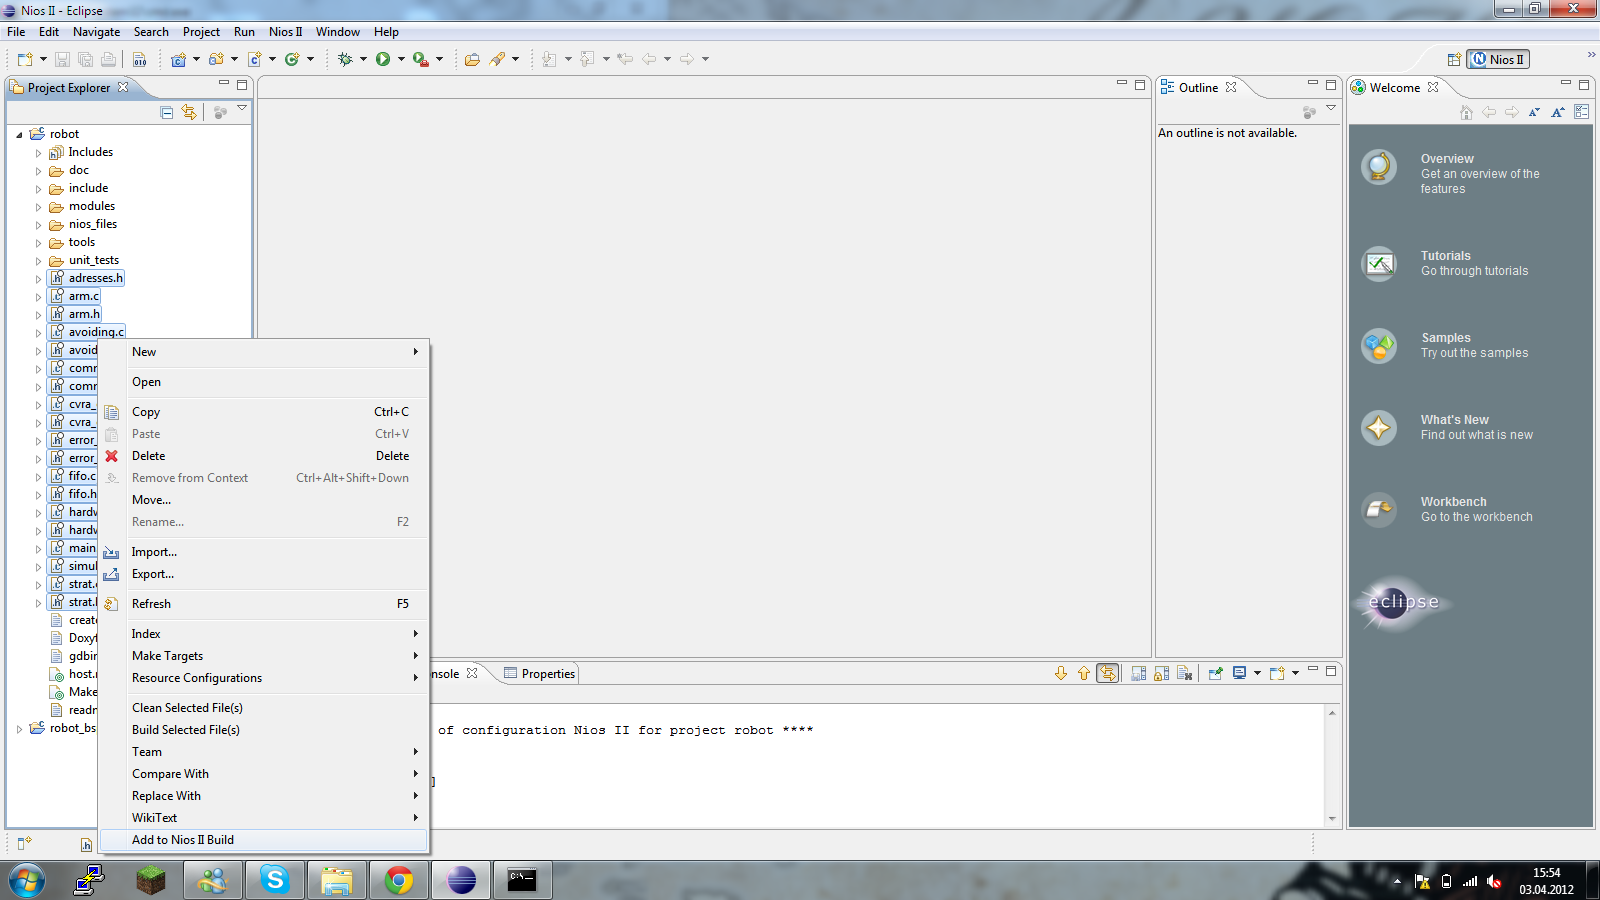
\includegraphics[width=0.8\textwidth]{4}
  \caption{Ajout des fichiers à la build.}
  \label{aa}
\end{figure}


Nous allons maintenant passer à la modification du Makefile. Si Eclipse affiche une erreur à la place du Makefille, faire click droit sur le
fichier et "Refresh...". 

Il faut trouver la ligne suivante :
\begin{lstlisting}[frame=trBL]
ALT_CFLAGS := 
\end{lstlisting}
Et la modifier en :
\begin{lstlisting}[frame=trBL]
ALT_CFLAGS := -DCOMPILE_ON_ROBOT
\end{lstlisting}
Ensuite trouver la ligne :
\begin{lstlisting}[frame=trBL]
ALT_INCLUDE_DIRS :=
\end{lstlisting}
Et la changer en :
\begin{lstlisting}[frame=trBL]
ALT_INCLUDE_DIRS := include/
ALT_INCLUDE_DIRS += modules/math/vect2 
ALT_INCLUDE_DIRS += odules/math/fixed_point 
ALT_INCLUDE_DIRS += modules/math/geometry
ALT_INCLUDE_DIRS += modules/cvra_adc 
ALT_INCLUDE_DIRS += modules/cvra_bldc modules/cvra_dc
ALT_INCLUDE_DIRS += modules/error 
ALT_INCLUDE_DIRS += modules/scheduler
ALT_INCLUDE_DIRS += modules/pid 
ALT_INCLUDE_DIRS += modules/quadramp 
ALT_INCLUDE_DIRS += modules/control_system_manager
ALT_INCLUDE_DIRS += modules/robot_system 
ALT_INCLUDE_DIRS += modules/position_manager 
ALT_INCLUDE_DIRS += modules/blocking_detection_manager
ALT_INCLUDE_DIRS += modules/trajectory_manager
ALT_INCLUDE_DIRS += modules/obstacle_avoidance
ALT_INCLUDE_DIRS += modules/couple_limiter 
ALT_INCLUDE_DIRS += modules/cvra_logger
\end{lstlisting}

\section{Installation des drivers pour le FIFO UART}
% Il faut ouvrir tools/fifoed_uart.zip et l'extraire dans "c:/altera/<version>/ip/user_components/fifoed_avalon_uart"

\section{Réglage du BSP}
La dernière chose à faire est de configurer le BSP. Pour ca faire un clic droit sur le
projet BSP et aller dans \"Nios II -> BSP editor\". Régler stderr sur le jtag\_uart et stdin et stdout sur commPC.

\section{Compilation et upload}
Pour compiler le projet le plus simple est de le faire en ligne de commande. Pour
ouvrir un shell, click droit sur le projet et ensuite "Nios II -> Nios II command shell". 
Un shell UNIX s'ouvre alors.



Pour compiler, faire
\begin{lstlisting}[frame=trBL]
> make
\end{lstlisting}

et pour programmer le microcontrolleur (compile automatiquement avant) :
\begin{lstlisting}[frame=trBL]
> make download-elf
\end{lstlisting}

\textbf{Attention :} Seule la RAM du microcontrolleur est programmée. Une fois la
version définitive (utilisée en match) terminée, consulter la section \ref{program-flash}
pour mettre le programme dans l'\textsc{EPCS}\footnote{Puce contenant la configuration du FPGA
et le programme pour le Nios II de façon persistante}.

\chapter{Debugging avec GDB}
Il est possible de debugger en utilisant GDB\footnote{GNU Debugger}. Pour cela il faut demarrer
un serveur GDB qui se chargera de faire la communication JTAG - GDB et ensuite démarrer gdb et se connecter
au serveur précedemment créé.

\section{Démarage du serveur gdb}
Pour démarrer le serveur GDB il faut ouvrir une console Nios II et taper la commande suivante :
\begin{lstlisting}[frame=trBL]
> nios2-gdb-server --tcpport 1234 --tcppersist
\end{lstlisting}
Cette commande va démarrer un serveur sur le port TCP 1234. Il se peut que
le firewall Windows se déclenche, dans ce cas il suffit d'autoriser la connexion.
Le texte suivant devrait alors s'afficher :
\begin{lstlisting}[frame=trBL]
Using cable "USB-Blaster [USB-0]", device 1, instance 0x00
Pausing target processor: OK
Listening on port 1234 for connection from GDB:
\end{lstlisting}

\section{Connexion au serveur}
Il faut maintenant ouvrir une nouvelle console Nios II, la première étant
occupée par le serveur. Dans celle ci taper :
\begin{lstlisting}[frame=trBL]
> nios2-elf-gdb
\end{lstlisting}
On se retrouve maintenant dans l'invite de commande GDB dans laquelle on
peut se connecter au serveur précédemment créé et transférer le programme
sur le robot (le programme s'appelle ici Procty.elf, il faut bien entendu
adapter la ligne de commande en cas de besoin).
\begin{lstlisting}[frame=trBL]
(gdb) target remote localhost:1234
(gdb) file Procty.elf
(gdb) load
\end{lstlisting}

\section{Arret et reprise du programme}
Pour reprendre l'éxécution du programme ou le démarrer si il vient d'être
téléchargé il faut utiliser la commande "continue".
\begin{lstlisting}[frame=trBL]
(gdb) continue
\end{lstlisting}
Pour mettre en pause le programme, il faut faire Ctrl+C. Pour le moment
les breakpoints ne sont pas supportés, il faudrait travailler dessus.\footnote{https://bitbucket.org/antoinealb/code-source-carte-robot-2011/issue/19}
A partir de là plusieurs commandes marchent :
\begin{lstlisting}[frame=trBL]
(gdb) backtrace # Affiche la stack actuelle du programme
(gdb) print a # Affiche la valeur de a
(gdb) print robot.isBlocked
\end{lstlisting}
\end{document}
